\documentclass{amsart}
\usepackage{amsmath}
\usepackage{amssymb}
\usepackage{tikz}

\begin{document}

    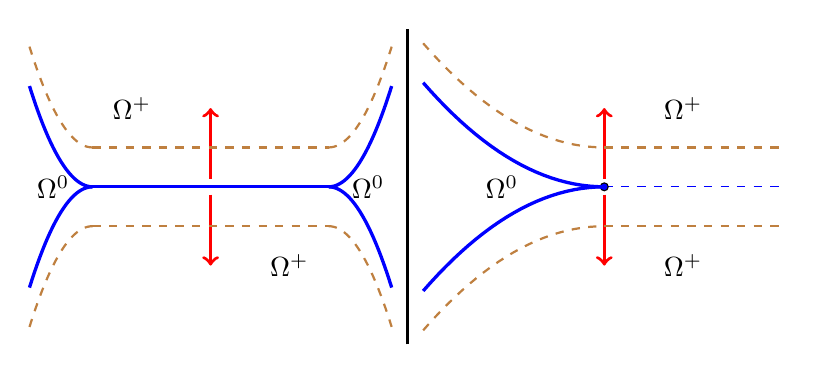
\begin{tikzpicture}

      % free boundary
      \draw[very thick, blue] (1,2) -- (4,2);
      \draw[very thick, blue, domain=0.2:1] plot (\x,{2*(\x -1)^2+2});
      \draw[very thick, blue, domain=0.2:1] plot (\x,{-2*(\x -1)^2+2});
      \draw[very thick, blue, domain=4:4.8] plot (\x,{2*(\x -4)^2+2});
      \draw[very thick, blue, domain=4:4.8] plot (\x,{-2*(\x -4)^2+2});

      % ker A
      \draw[very thick, red, ->] (2.5,2.1) -- (2.5,3);
      \draw[very thick, red, ->] (2.5,1.9) -- (2.5,1);

      % notation
      \draw (0.5,2) node{$\Omega^0$};
      \draw (4.5,2) node{$\Omega^0$};

      \draw (1.5,3) node{$\Omega^+$};
      \draw (3.5,1) node{$\Omega^+$};

      \draw[thick, brown, dashed] (1,2.5) -- (4,2.5);
      \draw[thick, brown, dashed, domain=0.2:1] plot (\x,{2*(\x -1)^2+2.5});
      \draw[thick, brown, dashed, domain=4:4.8] plot (\x,{2*(\x -4)^2+2.5});
      \draw[thick, brown, dashed] (1,1.5) -- (4,1.5);
      \draw[thick, brown, dashed, domain=0.2:1] plot (\x,{-2*(\x -1)^2+1.5});
      \draw[thick, brown, dashed, domain=4:4.8] plot (\x,{-2*(\x -4)^2+1.5});

      \draw[very thick] (5,0) -- (5,4); % boundary

      % Gamma 
      \draw[blue, thin, dashed] (7.5,2) -- (9.8,2);
      \draw[fill=blue,stroke=blue] (7.5,2) circle[radius = 0.05];
      \draw[very thick, blue, domain=5.2:7.5] plot (\x,{0.25*(\x-7.5)^2 + 2});
      \draw[very thick, blue, domain=5.2:7.5] plot (\x,{-0.25*(\x-7.5)^2 + 2});

      % ker A
      \draw[very thick, red, ->] (7.5,2.1) -- (7.5,3);
      \draw[very thick, red, ->] (7.5,1.9) -- (7.5,1);

      % notation
      \draw (6.2,2) node{$\Omega^0$};

      \draw (8.5,3) node{$\Omega^+$};
      \draw (8.5,1) node{$\Omega^+$};

      \draw[brown, thick, dashed] (7.5,2.5) -- (9.8,2.5);
      \draw[brown, thick, dashed] (7.5,1.5) -- (9.8,1.5);
      \draw[thick, brown, dashed, domain=5.2:7.5] plot (\x,{0.25*(\x-7.5)^2 + 2.5});
      \draw[thick, brown, dashed, domain=5.2:7.5] plot (\x,{-0.25*(\x-7.5)^2 + 1.5});

    \end{tikzpicture}

\end{document}